% DOC SETTINGS ===================================
\documentclass{article}
\usepackage[utf8]{inputenc}
\usepackage{steinmetz}
\usepackage{mathtools}  
\usepackage{multicol}
\usepackage{circuitikz}
\usepackage{listings}
\usepackage{geometry}
\usepackage{fancyhdr}
\pagestyle{fancy}
\lhead{ECE2214 Homework 1}
\rhead{Kavin Thirukonda 2021}
\fancyheadoffset{0mm}
 \geometry{
 a4paper,
 total={170mm,257mm},
 left=20mm,
 top=25mm,
 }
\mathtoolsset{showonlyrefs} 
\cfoot{}
% DOC SETTINGS ===================================
\begin{document}
\begin{enumerate}
\item Si is doped with 2$\cdot 10^{17}$ boron (B) $atoms/cm^3$ and 6$\cdot10^{17}$ phosphorus (P) $atoms/cm^3$
\begin{enumerate}
    \item Is this n-type or p-type and why?
    \begin{align}
        N_A &= 2\cdot 10^{17}\\
        N_D &= 6\cdot10^{17}\\
        N_D &> N_A
    \end{align}
    \begin{center}
        This is a \boxed{n-type} semiconductor because there is more phosphorus than there is boron which leads to there being more electrons as charge carriers than there is holes which makes it an n-type.
    \end{center}
    \item What are the electron and hole concentrations at 300K? (use $n_i = 10^{10} cm^{-3}$)
    \begin{align}
        p &= \frac{n_i^2}{N_D} =  \frac{(10^{10})^2}{6\cdot10^{17}} = \boxed{166.7}\\
        n &= \frac{n_i^2}{N_A} = \frac{(10^{10})^2}{2\cdot10^{17}} = \boxed{500}
    \end{align}
    \begin{center}
        Using the values from the initial problem and from the current problem we can calculate the electron and hole densities using the simple formulas shown above.
    \end{center}
    \item Calculate resistivity of Si doped with donor density of $N_D = 2 \cdot 10^{15}$ and $N_A = 0$ (use $n_i = 10^{10} cm^{-3}$; $\mu_n = 1320 cm^2/Vs$; $\mu_p = 460 cm^2/Vs$)
    \begin{align}
        p &= \frac{(10^{10})^2}{2\cdot10^{15}} = 50000\\
        n &= \frac{(10^{10})^2}{0} = undefined \approx 0 \quad ???\\
        \rho &= \frac{1}{en\mu_n + ep\mu_p} = \frac{1}{(1.6\cdot10^{-19})(0)(1320) + (1.6\cdot10^{-19})(50000)(460)} = \boxed{2.713\cdot 10^{11}}\\
    \end{align}
    \item In a Germanium semiconductor at T = 250K ($n_i = 1\cdot10^{12} cm^{-3}$), it is found that $p_o = 4n_o$ and that $N_d = 0$. Determine $p_o$, $n_o$, and $N_A$.
    \begin{align}
        n_o &= 5 \cdot 10^{11}\\
        p_o &=  N_A =  2 \cdot 10^{12}
    \end{align}
    \item Calculate the intrinsic carrier concentrations of these three bandgap materials at 300K: $Eg = 1.22eV$; and Eg = 0.66eV; where pre-factors are B = $1.08\cdot10^{31} K^{-3}\cdot cm^{-3}$ (1.12eV) and B = $2.31\cdot10^{30} K^{-3} \cdot cm^{-3}$ (0.66eV).
    \begin{align}
        n_i &= 6.72 \cdot 10^{9}\\
        n_i &= 2.3 \cdot 10^{13}\\
    \end{align}
\end{enumerate}
\newpage
\item
\begin{enumerate}
    \item Suppose a drift current density 5000 $A/cm^2$ present on the p-type side of a diode that has a resistivity of $2.5 \Omega\cdot cm$ at 300K (use $n_i = 1.5\cdot10^{10}cm^{-3}$ if needed). What is the electric field needed to support this drift current density?
    \begin{equation}
        \sigma = \frac{1}{2.5\Omega\cdot cm} = .4
    \end{equation}
    \begin{equation}
        E = \frac{5000}{.4} = 12500 
    \end{equation}
    \item A GaAs semiconductor resistor is doped with acceptor impurities at a concentration of of $Na = 10^{17}cm^{-3}$.  The cross-sectional area is $85\mu m^2$.  The current in the resistor is to be I = 20mA with 10V applied.  Determine the required length of the device. ($\mu_ p = 210 cm^2/Vs$).
    \begin{equation}
        1.4\cdot 10^{-3}
    \end{equation}
\end{enumerate}
\newpage
\item 
\begin{enumerate}
    \item The hole concentration in p-type GaAs is given by $p = 10^{16}\left(1 - \frac{x}{L}\right)cm^{-3}$ for $0 \leq x \leq L$ where L = $10\mu m$. The hole diffusion coefficient is 10 $cm^2/s$. Calcuate the hole diffusion current density at x = 5 $\mu m$. 
    \begin{align}
        p &= 10^{16}\left(1 - \frac{x}{L}\right)\\
        \Rightarrow \frac{dp}{dt} &= - \frac{1}{L}\\
        J_p &= -eD_p\frac{dp}{dt} = -(1.6 \cdot 10^{-19})(10)(-\frac{1}{L}) = \frac{1.6022 \cdot 10^{-20}}{5\cdot10^{-9}} = 3.2\cdot10^{-12}
    \end{align}
    \item The electron diffusion current density in a semiconductor is a constant and is given by $J_n= -2A/cm^2$.  The  electron  concentration  at x=  0  is n(0)  =  $10^{15}cm^{-3}$.  Calculate  the  electron concentration at $x= 20 \mu m$ if the material is Si with $D_n=30 cm^2/s$ $  (n_i= 1.5\cdot10^{10}cm^{-3})$
    \begin{equation}
        1.7\cdot10^{14}
    \end{equation}
\end{enumerate}
\newpage
\item
\begin{enumerate}
    \item A silicon p-n junction diode is designed to operate at T = 300K such that the diode current is 10 mA at a forward diode voltage of 0.65V.  The current density is not to exceed $20A/cm^2$ under this operating condition.  
    \begin{enumerate}
        \item Determine the reverse saturation current density of this diode:
        \begin{equation}
            J_s = \frac{J_D}{(e^{\frac{v_D}{V_T}}-1)} =   \frac{(20)}{(e^{\frac{(.65)}{(.026)}}-1)} = 2.78\cdot10^{-10}
        \end{equation}
        \item Determine the cross-section area of the diode:
            \begin{equation}
                A = \frac{10\cdot10^{-3}}{20} = 5 \cdot 10^{-4}
            \end{equation}
    \end{enumerate}
    \item Consider an ideal p-n junction diode operating in the forward bias region at 300K. Calculate the  change  in  diode  voltage that  will  cause  a  factor  of  10  increase  in  current  (same  reverse saturation current)? 
        \begin{equation}
            I_D = I_s(e^{\frac{v_D}{V_T}}-1) = (2.78\cdot10^{-10})(5\cdot 10^{-4})(e^{\frac{(.65)}{(.026)}}-1) = .010008681
        \end{equation}
        \begin{center}
            by multipling the $I_D$ value we just solved for with the equation we used to solve it we can obtain the forward voltage needed for the 10 times increase by multiplying $I_D$ by ten and solving.
        \end{center}
        \begin{equation}
            v_D = .026ln\left(\frac{.10008681}{(2.78\cdot10^{-10})(5\cdot 10^{-4})} + 1\right) = .71V       
        \end{equation}
        \begin{center}
            and therefore the change in voltage for ten times the current would be:
        \end{center}
        \begin{equation}
            \Delta v_D = .71 - .65 = .06V
        \end{equation}
\end{enumerate}
\newpage
\item Calculate the diode current $(I_D)$ and diode voltage $(V_D)$ from this circuit with iterative method (don’t assume voltage drop across diode)
\begin{center}
    \begin{circuitikz}
    \draw
    (0,0) to [R, l=$5\Omega$](2.5,0)
    to [R, l=$10\Omega$](5,0)
    to [diode, -] (5,-2.5)
    to [R, l=$10\Omega$](2.5,-2.5)
    to [short, -](0,-2.5)
    to [battery, l=$20V$, invert](0,0)
    (2.5,0) to [R, l=$20\Omega$](2.5,-2.5);
    \end{circuitikz}
    
    First we find the equivalent of this circuit and redraw using the values $R_{th} = 24\Omega$ and $V_{th} = 16V$
    
    \begin{circuitikz}
    \draw
    (0, -2.5) to [battery, l=16V, invert] (0,0)
    to [resistor, l=$24\Omega$](4, 0)
    to [diode, -] (4, -2.5)
    to [short, -] (0, -2.5);
    \end{circuitikz}
      
    Now we can try numbers for $v_D$ and work towards the value starting at .55 ($I_S = 2.8\cdot 10^{-10}$).    
\end{center}
\begin{equation}
    I_D = (2.8\cdot 10^{-10})(e^{\frac{(.55)}{(.026)}}-1)) = .43068
\end{equation}
\begin{center}
    this value is too small, now using a calculator I can further narrow down the value to achieve the source voltage and I get down to:
\end{center}
\begin{equation}
    v_D = .5825
\end{equation}
\begin{center}
    using this value of forward voltage the correct source value is only off by a factor a couple thousands.
\end{center}
\newpage
\item Find the Q-points $(I_{D1}, V_{D1})$ and $(I_{D2}, V_{D2})$ of these two diodes D1 and D2 of the circuit given below. Use constant voltage drop $V_{ON}= 0.7V$ at 300K (0.7V is needed for diode to be turned ON).



\begin{center}
    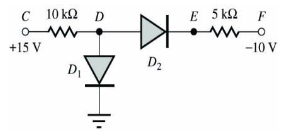
\includegraphics[width = .4\textwidth ]{p6.png}

    First take an educated guess that $D_1$ is OFF and $D_2$ is ON, the circuit can be redrawn like this:
    
    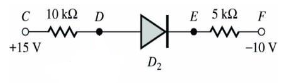
\includegraphics[width = .4\textwidth ]{p6-2.png}
\end{center}
\begin{equation}
    I_{D2} = \frac{25V - .07V}{15k\Omega} = 1.62mA\\
\end{equation}
\begin{center}
    Therefore the operating point of the two diodes $D_1$ and $D_2$ are:
\end{center}
\begin{align}
    (I_{D1}, V_{D1}) &= (1.62mA, 0.7V)\\  
    (I_{D2}, V_{D2}) &= (0A, -1.2V)
\end{align}
\newpage
\end{enumerate}
\end{document}
